\documentclass{ut-thesis}
\usepackage{graphicx} % Required for inserting images
\usepackage{amsmath}
\usepackage{cite}
\usepackage{amssymb}
\usepackage{amsfonts}

\title{Bayesian Optimization using Information Gain Acquisition Functions}
\author{Ruifan (Ricky) Wu}
\date{March 2025}

\begin{document}

\maketitle

\begin{abstract}
Bayesian Optimization (BO) has emerged as a powerful framework for optimizing expensive black-box functions commonly encountered in machine learning, engineering design, and scientific experimentation. Central to BO is the use of acquisition functions that guide the selection of candidate points by balancing exploration and exploitation. While improvement-based acquisition functions, such as Probability of Improvement (PI) and Expected Improvement (EI), have shown success in many applications, they often struggle in settings where the objective function is high-dimensional or multimodal.

This thesis focuses on entropy-based acquisition functions, which adopt an information-theoretic approach by explicitly aiming to reduce uncertainty about the location or the value of the global optimum. We provide a review of entropy-driven strategies, including Entropy Search (ES), Predictive Entropy Search (PES), and Max-value Entropy Search (MES), outlining their theoretical foundations and the approximation techniques used to enable tractable computation.

Through a series of numerical experiments, we compare the performance of entropy-based and improvement-based methods across various benchmark functions. Our results highlight the advantages of information gain acquisition functions in terms of sample efficiency and robustness, particularly in scenarios where function evaluations are extremely costly. 
\end{abstract}

\begin{acknowledgements}
This thesis is dedicated to my mentors, family, and friends who have supported me throughout my undergraduate journey. It has been a challenging yet transformative experience, and it is your encouragement and guidance that have shaped who I am today.

To my thesis supervisor and friend, Professor Justin J. Beland, thank you for the opportunity to work on this fascinating research topic and for your guidance throughout the project. I am deeply grateful for your patience in teaching me, from core academic concepts to the finer details of scholarly writing. Beyond your academic mentorship, your kindness and emotional support have helped me overcome the pressure in my graduating year. I couldn't dream of a better mentor.

To my friends Boyan Liang, Yuye Huang, Zhixiang Huang, Yujia Shi, Erxin Yan, and Yiling Ge, thank you all for being such wonderful companions throughout my undergraduate life. Your emotional support has meant more to me than words can express. Just as you’ve always had faith in me, I have faith in each of you. May we all shine in our own paths in life.

Lastly, to my parents, Zhihui Wu and Xiaoai Zhao, thank you for everything. I truly feel lucky to have grown up in an environment filled with support, respect, and love,that I have the motivation to dream and the power to explore my life with confidence and courage. 

Thanks to everyone I’ve met over the past five years—you’ve all made this a truly wonderful life journey. Thank you for being a part of my life.

\end{acknowledgements}

{\footnotesize\setlength{\parskip}{10pt}\tableofcontents}

{\footnotesize\setlength{\parskip}{10pt}\listoffigures}

\clearpage


\chapter{Introduction}

\section{Background}

In many real-world optimization problems, evaluating a solution can be computationally expensive, time-consuming, or resource-intensive. This is especially true in domains such as machine learning, drug discovery, materials design, and robotics, where each evaluation may involve training complex models, running detailed simulations, or conducting physical experiments\cite{berkenkamp2023bayesian}\cite{zhang2020bayesian}\cite{8539993}. Traditional optimization methods, ranging from exhaustive grid searches to heuristic-driven strategies, often become impractical in these settings.

To address these challenges, there is a growing need for optimization strategies that can make the most of limited evaluations while intelligently navigating complex, uncertain landscapes. One such approach is BO, which has emerged as a powerful framework for optimizing black-box functions with high evaluation costs. Rather than relying on large volumes of random or structured sampling, BO strategically selects evaluation points based on a surrogate model that captures uncertainty and guides the search process.

Central to the effectiveness of BO is the use of acquisition functions, which determine where to evaluate next by balancing the trade-off between exploring uncertain regions of the search space and exploiting areas that appear promising. Improvmentment based acquisition strategies, such as those based on expected improvement or confidence bounds, have demonstrated success in many practical applications. However, they can be limited in complex settings, particularly in high-dimensional or multimodal problems, where model predictions become unreliable or biased toward local optima.

In response, information-theoretic acquisition functions have gained attention for their ability to prioritize evaluations that reduce uncertainty about the location of the optimum itself. Rather than focusing solely on short-term gains, these methods seek to improve the model’s global understanding of the objective function, often leading to faster convergence and more efficient use of resources. This shift from improvement-based heuristics to uncertainty-reduction strategies has significant implications for applications constrained by budget, time, or experimental cost.

This thesis investigates the theoretical motivations and practical benefits of BO with information gain-based acquisition functions. By comparing these approaches with traditional improvement-based methods across a range of benchmarks, we aim to understand their relative performance in guiding sample-efficient optimization.

\section{Research Objective}

The objectives of this thesis project are

\begin{itemize}
    \item Construct entropy-based acquisition functions (i.e., Entropy Search, Predictive Entropy Search and Max Value Entropy Search) that can be used in a BO setting where we use the statistics from a GP posterior distribution to compute the search policy for ES, PES and/or MES.
    \item Compare the performance of these acquisition functions in a BO setting against other common acquisition functions such as the probability of improvement, expected improvement, lower confidence bound and/or Thompson sampling.
\end{itemize}

\section{Thesis Layout}
The remainder of this thesis is organized as follows:

In Chapter 2, we aim to review background information on the Gaussian Process(GP), BO, and based acquisition functions within BO Settings. 

In Chapter 3, we aim to review background information on the Entropy Based Search methods.

In Chapter 4, we aim to carry out numerical studies that explain the experiment motivation, experiment setting, and the analysis on the experiment results.


\chapter{Literature Review}

In this chapter, we reviewed the BO framework, which employs a GP as a surrogate model and utilizes an acquisition function to determine the next sampling point. A detailed description of GP can be found in text by Rasmusen and Williams\cite{rasmussen2006gaussian}, while for BO the reader can refer to the text by Garnett et al.\cite{garnett2023bayesian} for a comprehensive explanation.

\section{Gaussian Process Overview}

GPs are a powerful and widely used approach in BO for constructing surrogate models of hidden objective functions\cite{rasmussen2006gaussian}. More broadly, GPs offer a probabilistic framework that seamlessly integrates with Bayesian Inference, allowing the model to make predictions while quantifying uncertainty. This makes them particularly valuable in scenarios where evaluating the true objective function is costly and only a limited number of observations are available.

This section introduces the reader to several relevant aspects of GP with the Function Space view of GP mentioned.

Formally, a GP is defined as a collection of random variables, where any finite subset follows a joint Gaussian distribution. Rather than specifying a function explicitly, a GP characterizes a distribution over functions, enabling a probabilistic approach to modeling unknown functions\cite{rasmussen2006gaussian}.

The GP model is completely specified by its mean function and covariance function. We define the mean function m(x) and the covariance function $k(\mathbf{x},\mathbf{x'})$ of a real process $f(\mathbf{x})$ as

\begin{equation}
    m(\mathbf{x}) = \mathbb{E}[f(\mathbf{x})],
\end{equation}
and 
\begin{equation}
    k(\mathbf{x}, \mathbf{x}') = \mathbb{E}[(f(\mathbf{x}) - m(\mathbf{x}))(f(\mathbf{x}') - m(\mathbf{x}'))],
\end{equation}
Respectively, where the target function $f : \mathbf{x} \in \mathbb{R}^d \to \mathbb{R}_\infty$

We often use a compact notation of a GP with mean function m and covariance function $f(\mathbf{x},\mathbf{x'})$

\begin{equation}
    f\sim \mathcal{GP} (m,k)
\end{equation}

Normally, for notational simplicity, we take the mean function to be zero, and when the mean function is non-zero, the GP can be rewritten as the offset with a mean function of $\hat{f} - m$.

\subsection{Gaussian Process Prior}
In GP Regression, we wish to use a GP as a surrogate and realization of the true objective function. For the default model used to approximate the hidden objective function, we typically assume a zero mean function. The prior kernel (covariance) function captures the knowledge and assumptions we have regarding the hidden objective function. 

\subsubsection{Squared Exponential (RBF) Kernel}

The squared exponential (SE) kernel, also known as the Radial Basis Function (RBF) or Gaussian kernel, defines the covariance between two input points $\mathbf{x}$ and $\mathbf{x'}$  in GPs\cite{rasmussen2006gaussian}, which takes the form of
\begin{equation}
    k_{\text{SE}}(\mathbf{x}, \mathbf{x'}) = \sigma_f^2 \exp\left( -\frac{\|\mathbf{x} - \mathbf{x'}\|^2}{2\ell^2} \right).
\end{equation}
The \textbf{length-scale} (\(\ell\)) determines how quickly the function values change with respect to the input; a larger \(\ell\) leads to smoother, more slowly varying functions, whereas a smaller \(\ell\) allows the function to exhibit rapid, local fluctuations. On the other hand, the \textbf{signal variance} (\(\sigma_f^2\)) governs the overall magnitude of variation in the function's output, indicating how far the function values are expected to deviate from the mean. Together, these hyperparameters play a critical role in shaping the behavior of the function modeled by a GP, as shown in Figure \ref{fig:gp_samples}.

\begin{figure}[htbp]
    \centering
    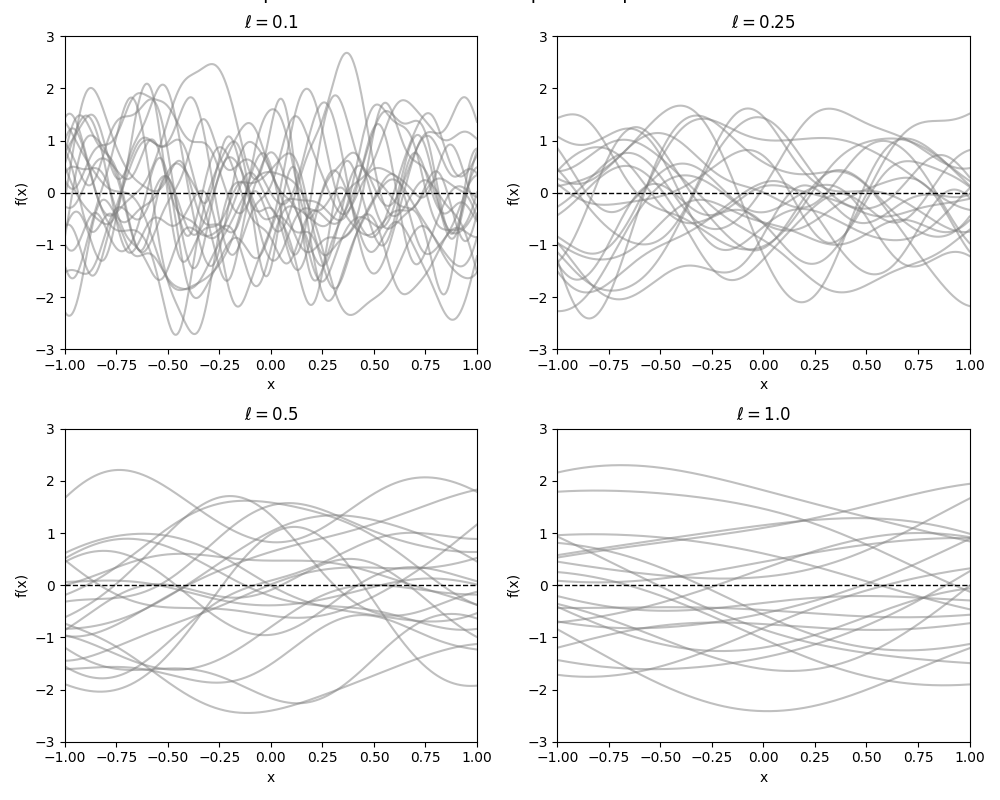
\includegraphics[width=0.7\textwidth]{rbf.png}
    \caption[Samples drawn from a Gaussian Process prior using the Squared Exponential kernel 
    with varying length-scale values \( \ell \) and fixed signal variance \( \sigma_f^2 = 1 \).]{Samples drawn from a GP prior using the Squared Exponential (SE) kernel 
    with varying length-scale values \( \ell \) and fixed signal variance \( \sigma_f^2 = 1 \). The dashed line indicates the zero prior mean.}
    \label{fig:gp_samples}
\end{figure}

\newpage
The standard SE kernel is isotropic, meaning it treats all input dimensions equally. However, with \textbf{Automatic Relevance Determination (ARD)}, each input dimension \( d \) is assigned its own length-scale (i.e. $\ell$  = ($\ell_1$, $\ell_2$, ...., $\ell_d$)) , resulting in an anisotropic kernel

\begin{equation}
    k_{\text{SE,ARD}}(\mathbf{x}, \mathbf{x'}) = \sigma_f^2 \exp\left( -\sum_{d=1}^{D} \frac{(x_d - x'_d)^2}{2\ell_d^2} \right).
\end{equation}

This ARD variant allows the model to infer the relevance of each input dimension, assigning longer length-scales to less relevant dimensions that result in little variation along those axes, and shorter length-scales to more relevant dimensions that allowing variation in those directions. This is shown in Figure \ref{fig:ard_kernel_bw}

The SE kernel is stationary, meaning it depends only on the Euclidean distance between points, ensuring translation invariance.

\begin{figure}[htbp]
    \centering
    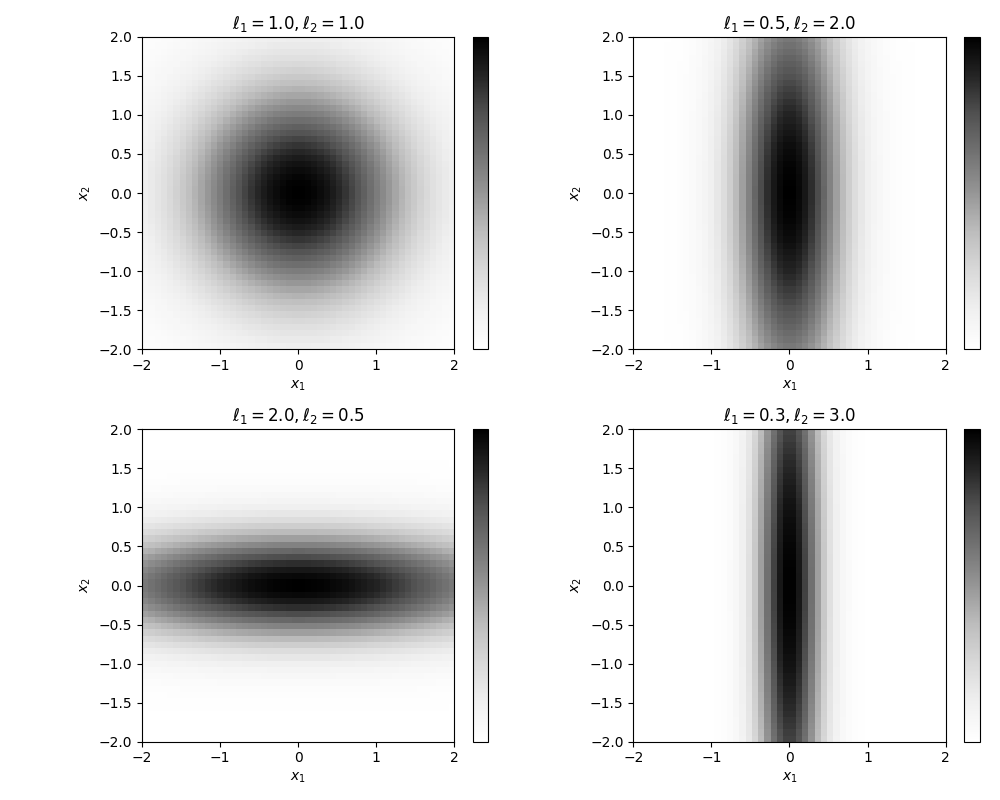
\includegraphics[width=0.85\textwidth]{rbf_with_ard.png}
    \caption[Visualization of the Squared Exponential kernel with Automatic Relevance Determination. ]
        {Grayscale visualization of the Squared Exponential (SE) kernel with Automatic Relevance Determination (ARD). 
        Each subplot illustrates kernel values \( k_{\text{SE,ARD}}(\mathbf{x}, \mathbf{x'}) \) for $\mathbf{x'} = (0, 0)$ under different dimension-specific length-scales. Shorter \( \ell_d \) indicates higher sensitivity along that input dimension.
    }
    \label{fig:ard_kernel_bw}
\end{figure}

\subsubsection{Matérn Kernel}
The Matérn kernel family introduces flexibility in smoothness assumptions through an additional parameter\cite{rasmussen2006gaussian}. Its general form for a distance $r = |x - x'|$ is

\begin{equation}
    k_{\mathrm{Mat\acute{e}rn}}(r)
= \sigma_f^2 \,\frac{2^{1-\nu}}{\Gamma(\nu)}
\left(\sqrt{2\nu}\,\frac{r}{\ell}\right)^{\nu}
K_{\nu}\!\left(\sqrt{2\nu}\,\frac{r}{\ell}\right)
\end{equation}

where $\nu > 0$ is a shape parameter, $\Gamma(\cdot)$ is the Gamma function, and $K_{\nu}(\cdot)$ is a modified Bessel function of the second kind. 

Like the RBF, $\ell$ is a length-scale and $\sigma_f^2$ a variance. The Matérn class includes the RBF as a limiting case – as $\nu \to \infty$, the Matérn kernel converges to the squared exponential form. 

Importantly, $\nu$ controls the smoothness of the functions in the GP prior. A GP with a Matérn covariance is $(\lfloor \nu \rfloor)$-times mean-square differentiable (i.e. roughly $\nu - 1$ times differentiable). In simpler terms, larger $\nu$ yields smoother functions. 

Common choices are half-integer values of $\nu$, for which the kernel has closed-form expressions:

\begin{itemize}
    \item $\nu = \frac{1}{2}$: The Ornstein–Uhlenbeck (OU) covariance
    
    \begin{equation}
    k(r) = \sigma_f^2 \exp\left( -\frac{r}{\ell}\right)
    \end{equation}

    Known as the exponential kernel. It produces very rough, non-differentiable sample paths that is continuous but not smooth. The OU kernel encodes an assumption that the function is unsmooth. The observations only inform a small neighborhood – points must be close to be strongly correlated

    \item $\nu = \frac{3}{2}$: Matérn-$3/2$ kernel

    \begin{equation}
        k_{\nu=\frac{3}{2}}(r) = \sigma_f^2 
        \left(1 + \sqrt{3}\,\frac{r}{\ell}\right)\exp\!\left(-\,\sqrt{3}\,\frac{r}{\ell}\right)
    \end{equation}

    which yields sample paths that are once differentiable. This kernel is smoother than OU, assuming moderate continuity in the function.

    \item $\nu = \frac{5}{2}$: Matérn-$5/2$ kernel

    \begin{equation}
        k_{\nu=\frac{5}{2}}(r) = \sigma_f^2 \left(1 + \sqrt{5}\,\frac{r}{\ell}+ \frac{5\,r^2}{3\,\ell^2}\right)\exp\!\left(-\sqrt{5}\,\frac{r}{\ell}\right).
    \end{equation}

    which yields twice differentiable sample paths. This is smoother than $\nu=3/2$ but still not as excessively smooth as RBF.
\end{itemize}

As shown in Figure~\ref{fig:matern_gp_samples}, increasing the parameter \( \nu \) in the Matérn kernel leads to smoother functions. Matérn-\( \frac{1}{2} \) produces highly non-smooth paths, while Matérn-\( \frac{3}{2} \) and \( \frac{5}{2} \) yield increasingly smooth trajectories. These kernels offer a flexible alternative to the RBF kernel, imposing less strict smoothness assumptions and better capturing functions with local variations.

\begin{figure}[htbp]
    \centering
    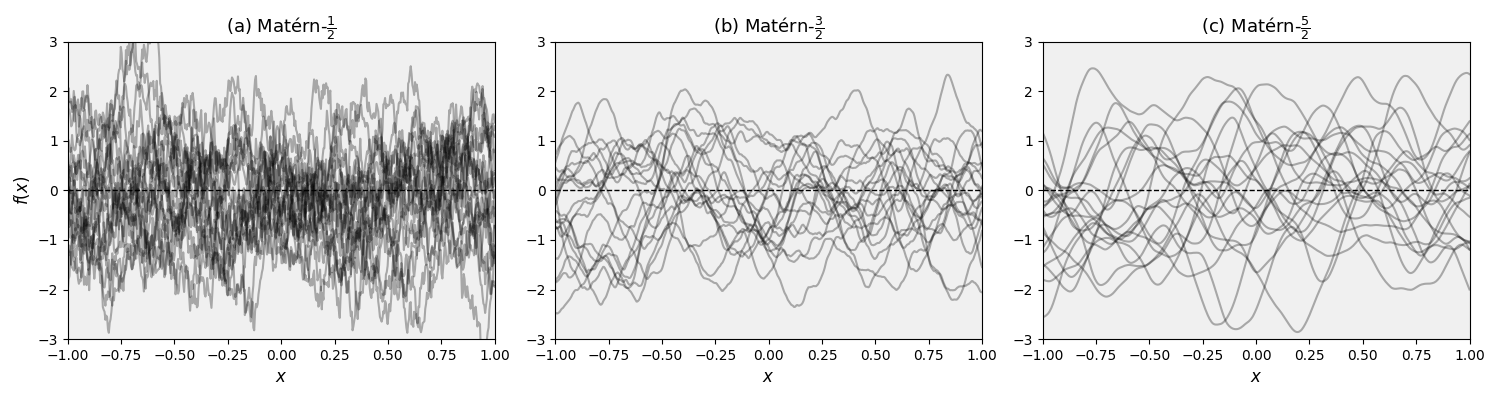
\includegraphics[width=\textwidth]{Matern.png}
    \caption[Gaussian Process samples with Matérn kernels]{
        Samples from GP priors using Matérn kernels with different smoothness levels \( \nu \).
        From left to right: (a) Matérn-\( \frac{1}{2} \), (b) Matérn-\( \frac{3}{2} \), and (c) Matérn-\( \frac{5}{2} \).
        As \( \nu \) increases, the functions become more smoother.
    }
    \label{fig:matern_gp_samples}
\end{figure}

\newpage
\subsubsection{Periodic Kernel}

The periodic kernel is designed to model functions that repeat with some fixed period\cite{mackay1998introduction}. One common form of a strictly periodic kernel is derived by mapping inputs through sine/cosine features. For input points $\mathbf{x}$ and $\mathbf{x'}$, a typical periodic kernel is

\begin{equation}
k_{\mathrm{Per}}(\mathbf{x}, \mathbf{x'})
= \sigma_f^2
\exp\!\left(
- \frac{2\,\sin^2\!\left(\tfrac{\pi\,\lvert \mathbf{x} - \mathbf{x'}\rvert}{p}\right)}{\ell^2}
\right).
\end{equation}
Here $p$ is the period of repetition, and $\ell$ is a length-scale parameter controlling how fast the covariance decays with misalignment in phase. Like other kernels, $\sigma_f^2$ scales the variance.

It defines a covariance that depends on $\sin^2(\frac{\pi|\mathbf{x}-\mathbf{x'}|}{p})$, which is $0$ when $\mathbf{x}$ and $\mathbf{x'}$ differ by an integer multiple of the period $p$. Thus $k_{\text{Per}}(\mathbf{x},\mathbf{x'}) = \sigma_f^2$ (maximum covariance) whenever $\mathbf{x'} = \mathbf{x} + \mathbf{mp}$ for some integer $m$, enforcing perfect periodicity of the GP prior with period $p$. The kernel is stationary on a wrapped domain (the circle of circumference $p$). Figure~\ref{fig:periodic_gp_samples} illustrates sample functions drawn from a GP prior with the periodic kernel, showing the repeating structure induced by the kernel.

\begin{figure}[htbp]
    \centering
    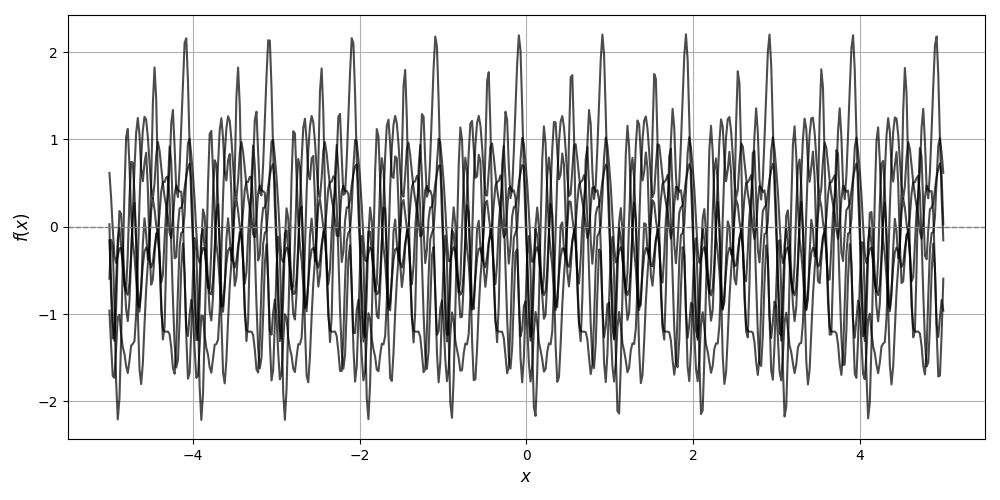
\includegraphics[width=0.7\textwidth]{periodic.png}
    \caption[Gaussian Process samples with periodic kernel]{
        Samples from a GP prior using a periodic kernel with period \( p = 1 \) and length-scale \( \ell = 0.3 \).
        The periodic kernel enforces strict periodicity, with maximum covariance when inputs differ by integer multiples of the period.
        Shorter length-scales result in sharper alignment around each phase, as seen in the repeating structure of the sample paths.
    }
    \label{fig:periodic_gp_samples}
\end{figure}

\newpage
\subsection{Gaussian Process Posterior}

A fundamental aspect of GPs is their inherent connection to Bayesian inference—the ability to make predictions and update beliefs as new information becomes available. In the GP posterior, new observations are incorporated to refine the model. In this section, we discuss the process of updating the GP posterior in both noise-free and noise-added observation scenarios.

\subsubsection{Posterior Distribution Derivation}

In GP regression, we consider a noise-free training dataset $D = \left( \mathbf{X}, \mathbf{Y} \right) = \left\{ \left( \mathbf{x}^{(i)}, f^{(i)} \right) \right\}_{i=1}^n $ and test points $ \mathbf{X_*}$, where the goal is to predict the function values $ f_* $ at $ \mathbf{X_*} $. Under a zero-mean GP prior, the joint prior distribution of training and test outputs follows

\begin{equation}
    \begin{bmatrix}
y \\[6pt]
f_*
\end{bmatrix}
\sim
\mathcal{N}\!\left(
0,\,
\begin{bmatrix}
k(\mathbf{X}, \mathbf{X}) & k(\mathbf{X}, \mathbf{X_*}) \\[6pt]
k(\mathbf{X_*}, \mathbf{X}) & k(\mathbf{X_*}, \mathbf{X_*})
\end{bmatrix}
\right).
\end{equation}


Here, $ k(\mathbf{X},\mathbf{X}) $ represents the covariance matrix for training inputs, $ k(\mathbf{X_*},\mathbf{X_*} ) $ for test inputs, and $ k(\mathbf{X},\mathbf{X_*}) $ the cross-covariance between them. The kernel function $ k $ defines prior assumptions on smoothness and continuity.

Applying Gaussian conditioning, the posterior mean and covariance functions become

\begin{equation}
    \mu_D(\mathbf{X_*}) = k(\mathbf{X_*}, \mathbf{X}) k(\mathbf{X}, \mathbf{X})^{-1} f
\end{equation}

\begin{equation}
    k_D(\mathbf{X_*}, \mathbf{X_*}) = k(\mathbf{X_*}, \mathbf{X_*}) - k(\mathbf{X_*}, \mathbf{X}) k(\mathbf{X}, \mathbf{X})^{-1} k(\mathbf{X}, \mathbf{X_*})
\end{equation}

The \textbf{posterior mean} \( \mu_D(\mathbf{X_*}) \) represents our best estimate of the function's value at \( \mathbf{X_*} \) given the observed data. It is a weighted linear combination of the training observations \( f \), where the weights are determined by the covariance between \( \mathbf{X_*} \) and the training inputs. This means the model uses nearby known data points to make predictions, assigning higher importance to observations that are more strongly correlated with \( \mathbf{X_*} \).

The \textbf{posterior covariance} \( k_D(\mathbf{X_*}, \mathbf{X_*}) \) describes the uncertainty in the predictions. 

This means that the model uncertainty is significantly reduced near observed data points, where it can rely on the support of known values to make confident predictions. In contrast, as we move further away from the observed points, the uncertainty in the predictions increases. This rising uncertainty reflects the model’s limited information about these regions, indicating less confidence in its predictions due to the lack of direct data support, as shown in Figure \ref{fig:gp_updates}.

\begin{figure}[htbp]
    \centering
    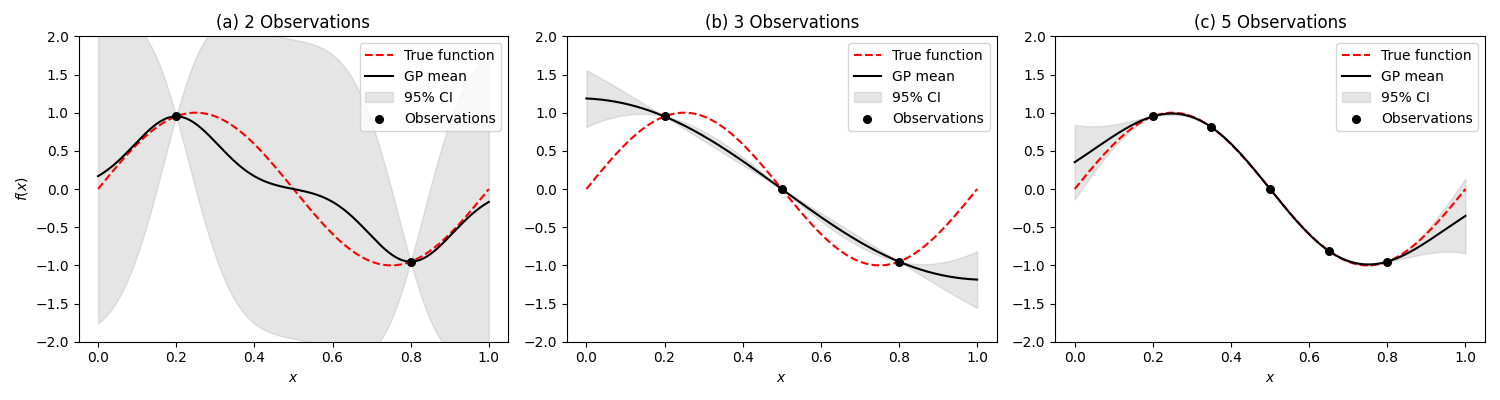
\includegraphics[width=\textwidth]{gp_post.png}
    \caption[Gaussian Process updates with added observations]{
        Illustration of GP posterior updates as more observations are added. 
        The true function (red dashed) is \( f(x) = \sin(2\pi x) \). 
        The GP mean (black line) and 95\% confidence interval (gray band) adjust with new data points.
        As the number of observations increases, the GP becomes more confident and accurate in regions close to the data.
    }
    \label{fig:gp_updates}
\end{figure}

\newpage
In practice, observations are often contaminated with noise. This is modeled as

\begin{equation}
    y = f(\mathbf{x}) + \varepsilon, \quad \varepsilon \sim \mathcal{N}(0, \nu^2),
\end{equation}

where \( \varepsilon \) represents Gaussian noise with variance \( \nu^2 \). As a result, the covariance of the observed outputs becomes

\begin{equation}
    \operatorname{cov}(y \mid \mathbf{X}) = k(\mathbf{X}, \mathbf{X}) + \nu^2 I,
\end{equation}

where the term \( \nu^2 I \) accounts for independent, identically distributed noise in each observation. Using this updated covariance structure, the posterior predictive distribution is also modified. The posterior mean function is given by

\begin{equation}
    \mu_D(\mathbf{X_*}) = k(\mathbf{X_*}, \mathbf{X}) \left[k(\mathbf{X}, \mathbf{X}) + \nu^2 I\right]^{-1} y,
\end{equation}

and the posterior covariance function becomes

\begin{equation}
    k_D(\mathbf{X_*}, \mathbf{X_*}) = k(\mathbf{X_*}, \mathbf{X_*}) - k(\mathbf{X_*}, \mathbf{X}) \left[k(\mathbf{X}, \mathbf{X}) + \nu^2 I\right]^{-1} k(\mathbf{X}, \mathbf{X_*}).
\end{equation}

In the presence of noise, the model no longer strictly interpolates the training data. Instead, it produces smoother predictions that account for the uncertainty introduced by the noise.

To determine suitable hyperparameters—such as the kernel's lengthscale and variance—it is common to maximize the log-marginal likelihood of the observed data

\begin{equation}
    \log p(y \mid \mathbf{X}) = -\frac{1}{2} y^{\top} (K + \sigma_n^2 I)^{-1} y - \frac{1}{2} \log \left|K + \sigma_n^2 I\right| - \frac{n}{2} \log 2\pi.
\end{equation}

\noindent
where \( K = k(\mathbf{X}, \mathbf{X}) \) is the kernel (covariance) matrix, and \( \sigma_n^2 \) is the noise variance.

This objective function strikes a balance between model fit and complexity. However, it is generally non-convex, so multiple optimization restarts are often employed to avoid getting trapped in poor local minima.


\section{Bayesian Optimization}

BO is a strategy for global optimization of expensive, black-box functions that lack closed-form expressions or easy derivatives\cite{garnett2023bayesian}\cite{frazier2018tutorial}. It addresses problems where each function evaluation is costly (e.g., time-consuming experiments or expensive simulations), so the goal is to find the global optimum in as few evaluations as possible. 

BO approaches this by building a probabilistic surrogate model of the objective function and using it to decide where to sample next. In essence, BO consists of two key components: (1) a Bayesian statistical model (usually a GP) that captures our current belief about the unknown function which had already introduced in the previous subsection, and (2) an acquisition function that uses this model to determine the next query point. This framework enables a principled exploration-exploitation trade-off – exploring uncertain regions while exploiting areas predicted to have high objective values.

One example can be shown in Figure~\ref{fig:bo_ei_iterations} that illustrates how the sample acquisition function, Expected Improvement, guides the search in BO. In early iterations, EI favors exploration in uncertain regions. As more points are observed, the GP model refines its estimate, and EI focuses around the likely minimum.

\begin{figure}[htbp]
    \centering
    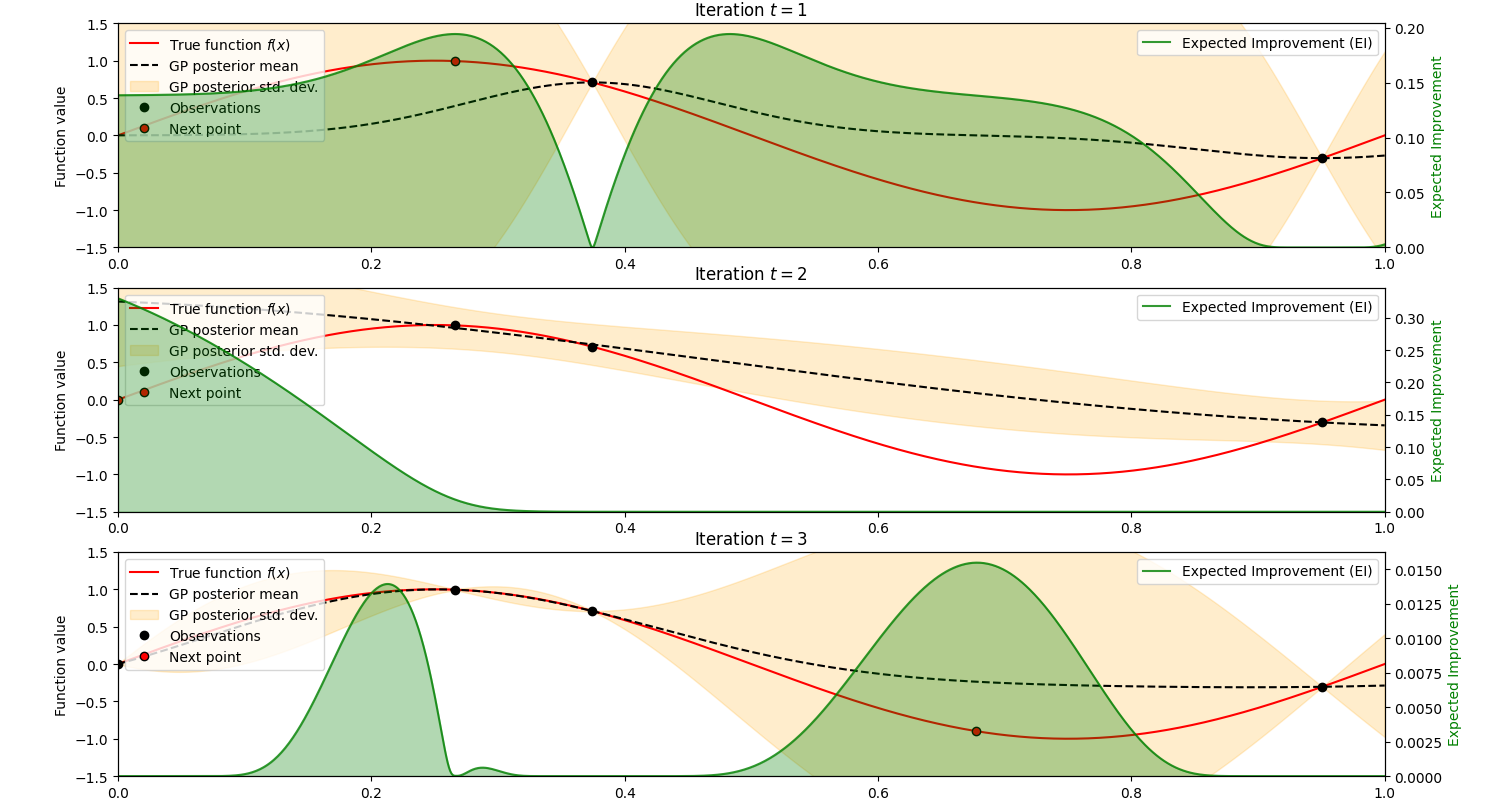
\includegraphics[width=0.95\textwidth]{Bo_visual.png}
    \caption[Bayesian Optimization with Expected Improvement]{
        Visualization of three iterations of BO using the Expected Improvement (EI) acquisition function. 
        The true function \( f(\mathbf{x}) \) (red) is unknown to the optimizer. At each step, a GP posterior (black dashed line with green uncertainty band) is updated based on observed data (black dots). 
        The EI acquisition function (light green curve) guides the selection of the next evaluation point (orange dot). 
        As the process continues, the GP becomes more confident near the optimum and EI shrinks in regions with low uncertainty or low expected gain.
    }
    \label{fig:bo_ei_iterations}
\end{figure}

\subsection{Improvement Based Acquisition Functions}

With a GP posterior in place, BO needs a policy to decide the next evaluation point. This role is played by \emph{acquisition functions} (also known as \emph{infill criteria} or \emph{utility functions}). 

An acquisition function $a(\mathbf{x})$ maps the GP’s predictive distribution at $x$ to a real value that reflects the utility of sampling at $x$. It is designed such that maximizing $a(\mathbf{x})$ (approximately) corresponds to selecting points that are expected to improve our objective. Crucially, acquisition functions depend only on the surrogate (GP) and not on the unknown true function---thus they are cheap to evaluate and can be optimized by standard methods.

Various acquisition functions have been proposed, each with different theoretical motivations. We focus here on three improvement-based choices: \emph{Probability of Improvement (PI)}, \emph{Expected Improvement (EI)}, and \emph{Gaussian Process Upper Confidence Bound (GP-UCB)}.

\subsubsection{Probability of Improvement (PI)}

The Probability of Improvement (PI) is one of the earliest BO acquisition functions\cite{kushner1964new}. PI chooses the next evaluation point by maximizing the probability that a new sample will outperform the current best observed value.

Let $f_n^* = \max \{ y_1, y_2, \dots, y_n \}$ be the best (maximum) outcome observed so far. The PI acquisition function is defined as:

\begin{equation}
    a_{\text{PI}}(\mathbf{x}) = \Pr\left( f(\mathbf{x}) > f_n^* + \xi \mid \mathcal{D}_n \right)
\end{equation}

where $\xi \geq 0$ is a slack (or exploration) parameter that can encourage exploration.

Assuming a GP posterior, $f(\mathbf{x}) \sim \mathcal{N}(\mu_n(\mathbf{x}), \sigma_n^2(\mathbf{x}))$, the probability can be evaluated in closed form as a Gaussian tail probability:

\begin{equation}
    a_{\text{PI}}(\mathbf{x}) = \Phi\left( \frac{\mu_n(\mathbf{x}) - (f_n^* + \xi)}{\sigma_n(\mathbf{x})} \right)
\end{equation}

where $\Phi(\cdot)$ denotes the standard normal cumulative distribution function.

The acquisition function $a_{\text{PI}}(\mathbf{x})$ tends to be high at points where the predicted mean significantly exceeds the current best value $f_n^*$, indicating a high likelihood of improvement. It can also be high in regions with large predictive uncertainty, which increases the chance of surpassing $f_n^*$.

PI only considers the probability of achieving any improvement, without accounting for the magnitude of the improvement. In other words, all improvements are treated equally, regardless of how substantial they are. PI may overly concentrate on regions that have a relatively high chance of minor improvement while ignoring areas with the potential for large improvements but lower probability. Consequently, PI often exhibits overly exploitative behavior, which may lead it to become stuck in local optima and fail to explore the search space adequately.

The exploration parameter $\xi$ (sometimes referred to as ``kappa'' in the literature) can partially address this issue. Increasing $\xi$ raises the threshold for improvement, thereby encouraging exploration. When $\xi = 0$, PI reduces to maximizing the probability $\Pr(f(\mathbf{x}) > f_n^*)$.

\subsubsection{Expected Improvement (EI)}
Expected Improvement is a refined acquisition function that overcomes the main limitation of PI by accounting for the magnitude of improvement. EI is defined as the expected gain in the objective value if sampling at $\mathbf{x}$, relative to the current best $f^*_n$\cite{mockus1975bayesian}\cite{mockus1989bayesian}. 

Formally, using the same $f^*_n = \max\{y_i \mid i \le n\}$ for a maximization problem, the improvement if we sample at $\mathbf{x}$ is 
\begin{equation}
    (f(\mathbf{x}) - f^*_n)_+ = \max\{0, f(\mathbf{x}) - f^*_n\}
\end{equation}

i.e., the amount by which $f(\mathbf{x})$ exceeds the incumbent best (or 0 if it does not). The expected improvement is then the posterior expectation of this quantity:
\begin{equation}
    a_{\mathrm{EI}}(\mathbf{x}) = \mathbb{E}_n\left[(f(\mathbf{x}) - f^*_n)_+\right]
\end{equation}
where $\mathbb{E}_n[\cdot]$ denotes expectation under the GP posterior $f(\mathbf{x}) \sim \mathcal{N}(\mu_n(\mathbf{x}), \sigma_n^2(\mathbf{x}))$. 

By taking the expectation, EI smoothly trades off the probability of improvement with the size of improvement. Points that have a small chance of greatly exceeding $f^*_n$ can thus score as well as points that will most likely yield a small improvement. One of the strengths of EI is that it has a closed-form expression for Gaussian posteriors. Using analytical integration by parts, one obtains:
\begin{equation}
    a_{\mathrm{EI}}(\mathbf{x}) = (\mu_n(\mathbf{x}) - f^*_n)\Phi(Z) + \sigma_n(\mathbf{x})\phi(Z)
\end{equation}
where $Z := \frac{\mu_n(\mathbf{\mathbf{x}}) - f^*_n}{\sigma_n(\mathbf{\mathbf{x}})}$, and $\phi(\cdot)$ and $\Phi(\cdot)$ are the standard normal PDF and CDF, respectively.


The first term, $(\mu_n(\mathbf{x}) - f^*_n)\Phi(Z)$, increases with a larger predicted mean $\mu_n(\mathbf{x})$ and reflects the exploitation component of the acquisition function, favoring points expected to outperform the current best. 

The second term, $\sigma_n(\mathbf{x})\phi(Z)$, grows with greater predictive uncertainty $\sigma_n(\mathbf{x})$ and captures the exploration component, encouraging sampling in less well-understood regions. 

Together, these terms ensure that EI naturally balances the trade-off between exploitation and exploration. If $\mu_n(\mathbf{x})$ is well below $f^*_n$, $Z$ is negative and $\Phi(Z)$ is small, but the second term $\sigma_n(\mathbf{x})\phi(Z)$ (approximately proportional to $\sigma_n(\mathbf{x})$ when $Z$ is small) ensures points with high uncertainty can still yield a decent EI. Conversely, if $\mu_n(\mathbf{x})$ is much larger than $f^*_n$, then even with small $\sigma_n(\mathbf{x})$, $Z$ is large and $\Phi(Z) \approx 1$, so $a_{\mathrm{EI}}(x) \approx \mu_n(\mathbf{x}) - f^*_n$—close to the predicted improvement.

This behavior encourages sampling in regions that are either promising in value or poorly understood, quantitatively embodying the exploration–exploitation trade-off. In fact, curves of constant EI in the $(\mu, \sigma)$ plane show an implicit trade-off: a point with moderate mean and high variance can equal the EI of a point with higher mean but lower variance.

\subsubsection{Gaussian Process Upper Confidence Bound (GP-UCB)}

The Upper Confidence Bound (UCB) acquisition function comes from a different perspective, the multi-armed bandit theory, and provides strong theoretical guarantees. GP-UCB is based on the principle of optimism in the face of uncertainty. 

The idea is to select the point that maximizes an upper confidence bound on the objective's value. Specifically, given the GP posterior $\mathcal{N}(\mu_n(\mathbf{x}), \sigma_n^2(\mathbf{x}))$, an upper $(1 - \delta)$-confidence bound for the unknown $f(\mathbf{x})$ can be written as $\mu_n(\mathbf{x}) + \sqrt{\beta_n}\sigma_n(\mathbf{x})$, where $\beta_n$ is a multiplier (dependent on $\delta$ and past data) that determines the confidence level. The GP-UCB policy chooses the next point as:
\begin{equation}
    \mathbf{x}_{n+1} = \arg\max_x \left\{ \mu_n(\mathbf{x}) + \sqrt{\beta_n}\sigma_n(\mathbf{x}) \right\}
\end{equation}

In other words, at each step it picks the location where the sum of the predictive mean and a scaled uncertainty is highest. The intuition is clear: $\mu_n(\mathbf{x})$ promotes points with high predicted reward (exploitation), while the $\sqrt{\beta_n}\sigma_n(\mathbf{x})$ term incentivizes exploration of uncertain points. 

By adjusting $\beta_n$ over time (typically a sequence growing at a rate related to $\ln n$), one can ensure that eventually the true optimum will be sampled with high probability. In fact, its proved that under an appropriate choice of $\beta_n$, the GP-UCB algorithm enjoys a sub-linear regret bound\cite{10.5555/3104322.3104451}.

GP-UCB has solid theoretical underpinnings: under certain smoothness conditions on the objective (captured by the GP prior), the sequence of points chosen by GP-UCB will converge to the global maximizer of $f(\mathbf{x})$ with high probability. This makes GP-UCB particularly attractive in scenarios where theoretical assurance is important (e.g., critical engineering systems or when designing algorithms with performance guarantees). In practice, a simplified version of GP-UCB often uses a constant $\beta$ (treated as a tunable parameter) and works well even without an increasing schedule, although the strict regret guarantees apply to the properly scheduled version. 

It is worth mentioning that UCB is typically described in terms of maximizing $f$; for minimization problems, one would use a \emph{Lower Confidence Bound} (LCB), defined as $\mu_n(\mathbf{x}) - \sqrt{\beta_n}\sigma_n(\mathbf{x})$. The theoretical property of eventual convergence holds analogously for the minimization case.



\chapter{Entropy Based Search Policies}

\section{Introduction}

Information-theoretic acquisition functions take a different approach: rather than directly optimizing an expected objective improvement or an upper bound, they aim to reduce uncertainty about the location of the global optimum. ES, PES, and MES are three such methods. They choose the next sample to maximally gain information about the argmax of $f(\mathbf{x})$, as quantified by entropy. These methods are more complex and computationally intense, but conceptually powerful.

This chapter intends to investigate the performance of the entropy-based acquisition functions compared to improvement based methods.

\section{Background}

\subsection{Information Gain In Bayesian Optimization}
Entropy is a fundamental concept from information theory that quantifies uncertainty in a probability distribution. Entropy $H[p]$ 
is defined as the negative expected log-probability of outcomes\cite{6773024}:
\begin{equation}
    H[p] = -\sum_i p_i \log p_i
\end{equation}
Intuitively, entropy measures the “spread” or unpredictability of a distribution, where a high entropy value indicates great uncertainty. For continuous distributions, a well-defined analog is the relative entropy or Kullback-Leibler (KL) divergence with respect to a reference measure\cite{kullback1968information}
\begin{equation}
    D_{\mathrm{KL}}(P \| Q) = \int_{-\infty}^{\infty} p(\mathbf{x}) \log \left( \frac{p(\mathbf{x})}{q(\mathbf{x})} \right) \, d\mathbf{x}
\end{equation}

Entropy’s interpretation as a measure of information content makes it a natural choice for guiding learning algorithms: reductions in entropy correspond to gains in information. In Bayesian terms, the expected information gain from an experiment can be quantified by the drop in entropy of the posterior distribution relative to the prior.


\subsection{Approximation Technique}
Entropy-based search methods in BO aim to select query points that maximize the expected information gain about the global optimum. However, calculating this information gain often involves complex integrals over high-dimensional distributions, which are analytically intractable. 

This is where approximation techniques become essential—they make the computation feasible by approximating difficult terms like the posterior over the global optimum or the expected reduction in entropy. 

\subsubsection{Monte Carlo Estimation}

Monte Carlo (MC) methods are widely used to approximate the expectations defining the acquisition. The idea is to sample from the GP posterior to approximate the distribution of the optimum\cite{robert2004monte}. 

The mutual information is then estimated by averaging entropy computations over these samples. The accuracy of MC integration improves with more samples at the cost of runtime. A trade-off arises: finer accuracy vs. computational cost. 

Typically a few thousand function samples may be needed for stable estimates in high dimensions, which is expensive but still far cheaper than a brute-force integration over a continuous domain. Techniques like importance sampling can sometimes improve efficiency by focusing samples in informative regions.

\subsubsection{Expectation Propagation}

Expectation Propagation (EP) is a deterministic approximation algorithm designed to estimate posterior distributions in probabilistic models where exact inference is computationally intractable\cite{minka2001expectation}. Unlike sampling-based methods such as Markov Chain Monte Carlo (MCMC), EP iteratively constructs a tractable approximation to the true posterior by minimizing the KL divergence in a local and moment-matching manner. 

The central idea behind EP is to approximate each non-conjugate factor in the posterior with a simpler, tractable distribution, usually chosen from the exponential family such as Gaussians. The result is an efficient inference scheme that maintains computational tractability while offering accurate approximations to posterior moments, particularly in models like GPs where analytic treatment of the prior is feasible but likelihoods may be non-Gaussian.

Given a probabilistic model with latent variables $\mathbf{z}$ and a set of observations $\mathcal{D} = \{x_i, y_i\}_{i=1}^n$, the true posterior is expressed as
\begin{equation}
    p(\mathbf{z} \mid \mathcal{D}) = \frac{1}{Z} p(\mathbf{z}) \prod_{i=1}^N p(y_i \mid z_i)
\end{equation}
where $p(\mathbf{z})$ is the prior and $p(y_i \mid z_i)$ are the likelihood terms. EP approximates this posterior using a simpler distribution
\begin{equation}
    q(\mathbf{z}) \propto p(\mathbf{z}) \prod_{i=1}^N \tilde{t}_i(z_i)
\end{equation}
where each $\tilde{t}_i(z_i)$ is a Gaussian site function approximating the original likelihood term. This ensures that the product $q(\mathbf{z})$ remains Gaussian and tractable, enabling efficient computation of marginals and moments.

The EP algorithm proceeds by iteratively updating each site factor. For a given site $i$, EP temporarily removes the site from the approximate posterior to form a \emph{cavity distribution}
\begin{equation}
    q^{\setminus i}(z_i) \propto \frac{q(z_i)}{\tilde{t}_i(z_i)}
\end{equation}
which captures the influence of all other factors. This cavity distribution is then multiplied by the original factor $p(y_i \mid z_i)$ to form a \emph{tilted distribution}
\begin{equation}
    \hat{p}(z_i) \propto q^{\setminus i}(z_i) \cdot p(y_i \mid z_i)
\end{equation}

Since $\hat{p}(z_i)$ may no longer be Gaussian, EP approximates it with a Gaussian distribution by matching the first and second moments (mean and variance). The updated moments are then used to compute new site parameters such that when recombined with the cavity distribution, the resulting marginal matches the tilted distribution in terms of these moments. 

EP is well-suited for models like Gaussian Process classification, where the prior $p(\mathbf{f})$ is Gaussian but the likelihood—such as the probit likelihood $\Phi(y_i f_i)$—is not. In such cases, EP approximates each likelihood term with a Gaussian, enabling closed-form posterior inference. This is crucial for applications like BO, where one needs accurate estimates of the marginal predictive distribution $p(y \mid \mathbf{x}, \mathcal{D})$ to compute acquisition functions such as Expected Improvement or entropy-based criteria. EP also plays an important role in entropy-based BO strategies such as Entropy Search and Predictive Entropy Search, where it enables tractable approximations of mutual information or expected information gain under GP priors.

\subsubsection{Gumbel Sampling}

Gumbel-based sampling which provides a tractable approximation for distribution of global maximum under certain assumptions\cite{wang2017max}. 

Specifically, when considering a finite set of input locations \( \{\mathbf{x_1}, \mathbf{x_2}, \dots, \mathbf{x_n}\} \subset \mathcal{X} \), and assuming the posterior predictive distribution of the GP at these locations yields independent function values \( f(\mathbf{x}_i) \sim \mathcal{N}(\mu_i, \sigma_i^2) \), the distribution of the maximum \( y^* \) over this set can be approximated using extreme value theory.

The key idea is that the maximum of a finite set of i.i.d. or weakly dependent Gaussian variables converges to a \textit{Gumbel distribution} in the limit. For finite \( n \), one can approximate the distribution of \( y^* \) as:
\begin{equation}
    p(y^*) \approx \text{Gumbel}(\mu, \beta)
\end{equation}
where the location and scale parameters \( \mu \) and \( \beta \) can be estimated empirically from samples of \( \max_i f(\textbf{x}_i) \), or via analytical approximations when available. Given this approximation, one can efficiently generate samples \( \{ y_j^* \}_{j=1}^M \sim p(y^*) \) without drawing full posterior function realizations.

These samples can then be used to compute mutual information terms of the form:
\begin{equation}
I(f(\mathbf{x}); y^*) = H(f(\mathbf{x})) - \mathbb{E}_{y^*}[H(f(\mathbf{x}) \mid y^*)]    
\end{equation}
where \( H(f(\mathbf{x})) \) is the entropy of the GP marginal at \( x \), and the conditional entropy \( H(f(\mathbf{x}) \mid y^*) \) is given by the entropy of a Gaussian truncated above \( y^* \):
\begin{equation}
    H(f(\mathbf{x}) \mid y^*) = \frac{1}{2} \log(2\pi e \sigma^2(\mathbf{x})) - \frac{\phi(z)}{2\Phi(z)} \cdot z
\end{equation}
with \( z = \frac{y^* - \mu(\mathbf{x})}{\sigma(\mathbf{x})} \), and \( \phi \), \( \Phi \) denoting the standard normal PDF and CDF, respectively. Averaging over the \( y^*_j \) samples gives an efficient and scalable entropy approximation.

Compared to standard Monte Carlo integration over function samples, this method significantly reduces computational cost while still capturing key aspects of the distribution of the optimum. However, the independence assumption may degrade the quality of approximation when posterior correlations are non-negligible.


\section{Entropy-based search methods}

\subsection{Entropy Search (ES)}

ES is a landmark algorithm that embodies an information-theoretic approach to BO\cite{hennig2012entropy}.  ES begins by defining a probability distribution \( p(\mathbf{x}^* \mid D_n) \) over the location of the global optimum \( x^* \) (typically the minimizer or maximizer of an unknown function), given the current data \( D_n \). This distribution captures the algorithm’s uncertainty about the location of the true optimum.

The acquisition function in ES is defined as the expected reduction in the entropy of this distribution after a hypothetical evaluation at a candidate point \( \mathbf{x} \). Formally, it is expressed as:
\begin{equation}
    \alpha_{\text{ES}}(\mathbf{x}) = H[p(\mathbf{x}^* \mid D_n)] - \mathbb{E}_{y \sim p(y \mid D_n, x)} \left[ H[p(\mathbf{x}^* \mid D_n \cup \{(\mathbf{x}, y)\})] \right]
\end{equation}

where \( H[\cdot] \) denotes the entropy. The first term \( H[p(\mathbf{x}^* \mid D_n)] \) represents the current uncertainty about the optimizer and is constant with respect to \( \mathbf{x} \). The second term is the expected residual uncertainty after observing a new function value \( y = f(\mathbf{x}) \), averaged over the predictive distribution of \( y \) at \( \mathbf{x} \). By maximizing \( \alpha_{\text{ES}}(\textbf{x}) \), the algorithm selects the evaluation point expected to yield the greatest information gain about the location of the global optimum.

Equivalently, ES seeks to maximize the mutual information between the new observation and the unknown optimum location \( \mathbf{x}^* \), a perspective that was emphasized in subsequent work.

In practice, computing \( p(\mathbf{x}^* \mid D_n) \) exactly is intractable because it involves reasoning about the argmax of a random function. ES addresses this by modeling the unknown function with a GP surrogate and approximating the optimizer distribution using methods such as Monte Carlo simulation or Expectation Propagation.

To make the optimization computationally feasible, ES often incorporates a pre-filtering step using simpler acquisition functions like PI to narrow down the candidate set before applying the full ES acquisition calculation. This helps manage computational cost, especially in high-dimensional or expensive-to-evaluate problems.

Entropy is measured in a relative sense using the negative KL divergence from a uniform reference distribution over the domain. This means that a uniform belief (i.e., complete uncertainty) incurs the highest loss, and as the optimizer distribution becomes more concentrated (i.e., entropy decreases), the loss diminishes. ES thus selects query points expected to maximally reduce this loss, or equivalently, to maximally increase information about \( x^* \).

\subsection{Predictive Entropy Search (PES)}

Predictive Entropy Search (PES) builds upon the same core idea as Entropy Search (ES), but introduces a crucial theoretical reframing to make the acquisition function significantly more tractable to compute\cite{hernandez2014predictive}. 

The key insight in Predictive Entropy Search (PES) is to exploit the symmetry of mutual information: the mutual information between the location of the global minimizer \( \mathbf{x}^* \) and a new observation \( y \) can be expressed in two equivalent ways. One formulation, as in Entropy Search (ES), defines it as the expected reduction in the entropy of the posterior distribution over the minimizer \( p(\mathbf{x}^* \mid D_n) \) after observing \( y \). The alternative, used in PES, interprets it as the expected reduction in the entropy of the predictive distribution \( p(y \mid D_n, \mathbf{x}) \) after conditioning on knowledge of \( \mathbf{x}^* \). These perspectives yield the same mutual information but differ in computational tractability and implementation.

The ES acquisition function \( \alpha_{\text{ES}}(\mathbf{x}) \) can be rewritten in a mathematically equivalent but computationally simplified “predictive” form through algebraic manipulation:

\begin{equation}
    \alpha_{\text{PES}}(\mathbf{x}) = H[p(y \mid D_n, \mathbf{x})] - \mathbb{E}_{\mathbf{x}^* \sim p(\mathbf{x}^* \mid D_n)} \left[ H[p(y \mid D_n, \mathbf{x}, \mathbf{x}^*)] \right]
\end{equation}

where \( H[\cdot] \) denotes entropy, and the expectation is now taken over samples of \( \mathbf{x}^* \) from the current belief. This formulation swaps the integration order compared to ES, avoiding the need to recompute the posterior over \( \mathbf{x}^* \) for every possible observation \( y \). Instead, PES samples plausible optima \( \mathbf{x}^* \sim p(\mathbf{x}^* \mid D_n) \) and computes the information gain that a query at \( \mathbf{x} \) would provide under each hypothesized true optimum.

This reframing makes PES much more computationally efficient. In practice, PES approximates \( p(\mathbf{x}^* \mid D_n) \) by drawing samples from the posterior GP, often via Monte Carlo simulation (e.g., drawing GP function realizations and computing their argmax). To maintain tractability, PES also supports other approximation methods such as Expectation Propagation for certain conditional entropy computations.

As with ES, computing the PES acquisition function can be expensive in high-dimensional or large-data settings. To mitigate this, PES implementations often include a pre-filtering step using simpler utility functions like EI or PI to select a small set of promising candidate points for full evaluation under the PES criterion.

PES retains the key advantage of ES, explicitly maximizing the mutual information between the next query and the global optimum, but it does so in a more computationally efficient manner by focusing on the entropy of the predictive observation space rather than the belief over the optimizer.


\subsection{Max Entropy Search (MES)}

Max-value Entropy Search (MES) is an information-theoretic acquisition strategy that selects query points by maximizing the mutual information between a potential observation and the unknown optimum value \( y^* = \max_{x} f(\mathbf{x}) \). By shifting the focus from the location of the optimum \( \mathbf{x}^* \) to the scalar output \( y^* \), MES avoids high-dimensional entropy estimation and significantly improves computational tractability.

Formally, MES selects the next evaluation point \( x \) by maximizing:
\[
\alpha_{\text{MES}}(\mathbf{\mathbf{x}}) = I(f(\mathbf{x}); y^* \mid \mathcal{D}_n),
\]
where \( \mathcal{D}_n \) denotes the current set of observations. This mutual information can be expressed as a difference in entropies:
\[
\alpha_{\text{MES}}(\mathbf{x}) = \mathcal{H}(f(\mathbf{x}) \mid \mathcal{D}_n) - \mathbb{E}_{y^*}[\mathcal{H}(f(\mathbf{x}) \mid y^*, \mathcal{D}_n)],
\]
where \( \mathcal{H} \) denotes differential entropy. The second term corresponds to the expected entropy of \( f(\mathbf{x}) \) conditioned on a given value of the maximum, effectively treating \( y^* \) as a threshold.

To approximate the distribution of \( y^* \), MES employs Gumbel-based sampling methods over the posterior of the GP surrogate. For further efficiency, candidate points may be pre-filtered using lightweight heuristics before computing the acquisition value.

MES is particularly well-suited for high-dimensional settings due to its reduced reliance on input-space sampling. It has also been shown to admit theoretical regret bounds, marking a significant development in the formal understanding of information-theoretic optimization methods.




\chapter{Numerical Studies}

To systematically evaluate the performance of various acquisition strategies in BO, we developed a controlled experimental framework using PyTorch and GPyTorch. The experiment compared six acquisition functions: LCB, EI, PI, ES, PES, and MES.

For each acquisition function, we assessed performance across varying problem dimensionalities (5, 10, and 20 dimensions) and tested them against several standard benchmark objective functions, including Rosenbrock, Ackley, and Schwefel. This setup allows us to analyze how each acquisition strategy scales with complexity and generalizes across different optimization landscapes.

\section{Experiment Setup}

A complete BO framework was implemented to support systematic experimentation under controlled conditions. For each experimental run, the optimization process begins with an initial training dataset generated by sampling 20 points randomly from a bounded domain of [-1, 1]. Gaussian noise $\sigma^2 = 0.01$  is added to simulate the observation noises.

The BO framework trains a GP model as the surrogate for the unknown objective function for each round of iteration. The GP model is trained via exact marginal log likelihood, using the LBFGS optimizer across 10 iterations to ensure convergence. In each BO iteration, the acquisition function is optimized to identify the next evaluation point, which is then queried using the true objective function. The resulting observation is appended to the training set, and the GP model is subsequently retrained to incorporate the new information.

This iterative process is repeated for 200 iterations, during which relevant metrics such as the best observed value, the number of improvements are recorded.

Each acquisition function was evaluated independently over ten experimental runs to account for stochastic variability and ensure statistical robustness. For each run, the initial training set was held fixed across all acquisition functions to ensure a fair comparison. Each acquisition function began its optimization with 100 pre-selected candidate points.

In the constructed acquisition functions for the experiment, the Lower Confidence Bound (LCB) and Probability of Improvement (PI) acquisition functions, the exploration parameter $\kappa$ was set to 0.01. Both Entropy Search and Predictive Entropy Search utilize PI as an utility function for pre-filtering and Monte Carlo Sampling as the approximation method, while Max Entropy Search use gumble sampling for approximation.
 

\section{Result And Analysis}

\begin{figure}[!t]
    \centering
    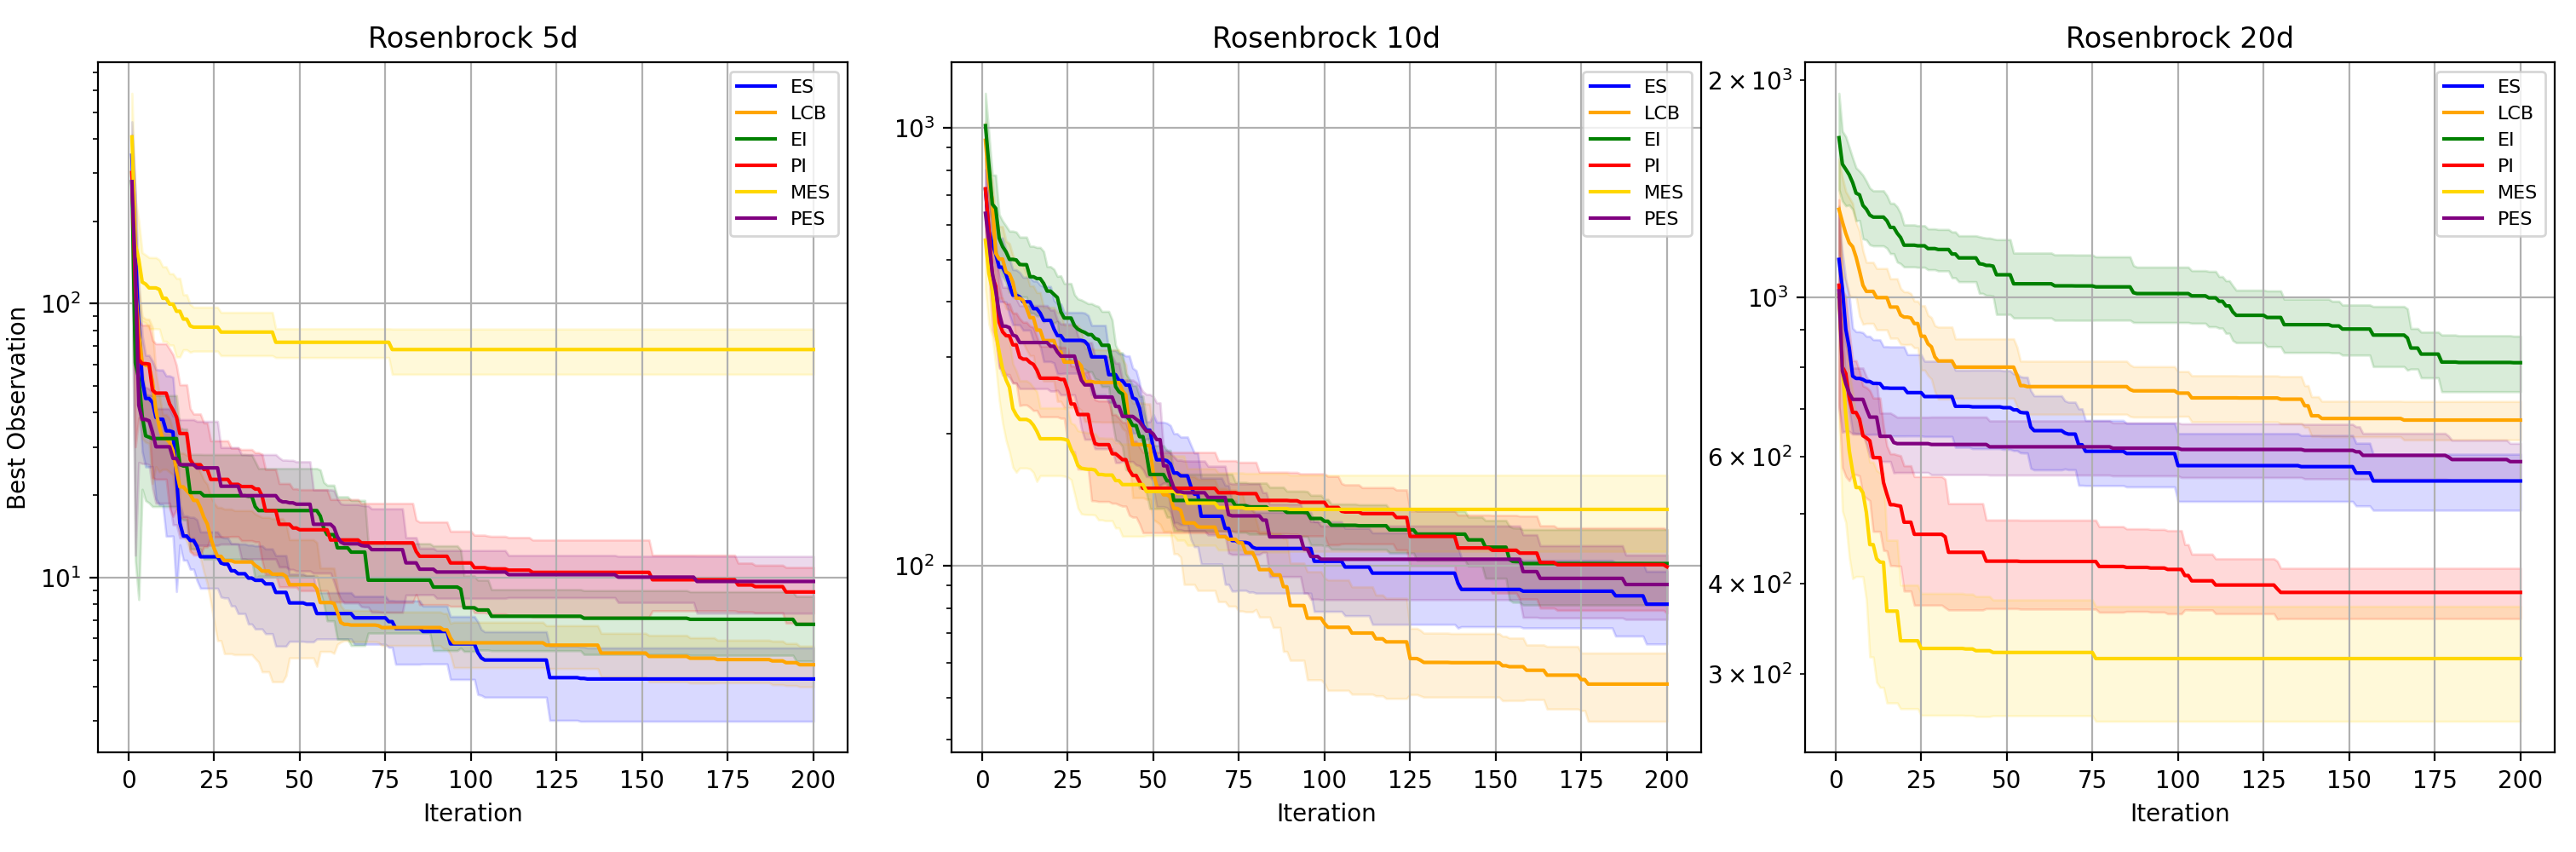
\includegraphics[width=\textwidth]{rosenbrock 51020d.png}
    \caption[Acquisition function comparison on Rosenbrock Function with different dimension]{Performance comparison of six acquisition functions (ES, LCB, EI, PI, MES, PES) on the Rosenbrock function in 5, 10, and 20 dimensions. The y-axis shows the best function value found so far, averaged over multiple runs, with shaded regions indicating 95\% confidence interval}
    \label{fig:rosenbrock_comparison}
\end{figure}

To evaluate the scalability of acquisition strategies, we assess their performance on the Rosenbrock function across 5, 10, and 20 dimensions. Figure~\ref{fig:rosenbrock_comparison} presents the best observed values over 200 iterations, averaged across trials, with shaded regions representing 95\% confidence interval.

Across all dimensions, PES and MES demonstrate superior performance, particularly in higher dimensions. Notably, both methods exhibit a steep initial decline in objective values, reflecting an accelerated convergence rate during early iterations. This rapid improvement suggests more efficient exploration and exploitation in the initial optimization phase.

In 5D, all methods converge reasonably well; however, PES and MES attain lower objective values more rapidly than EI and LCB, which display more gradual convergence. In 10D and 20D, the performance gap widens. Entropy-based methods maintain steady improvement, while EI and UCB plateau earlier, indicating diminishing effectiveness in higher-dimensional search spaces.

These results highlight the robustness and scalability of entropy-based acquisition functions. Their ability to capture global uncertainty contributes to faster convergence and improved performance as dimensionality increases, making them especially effective for high-dimensional BO.

\begin{figure}[!t]
    \centering
    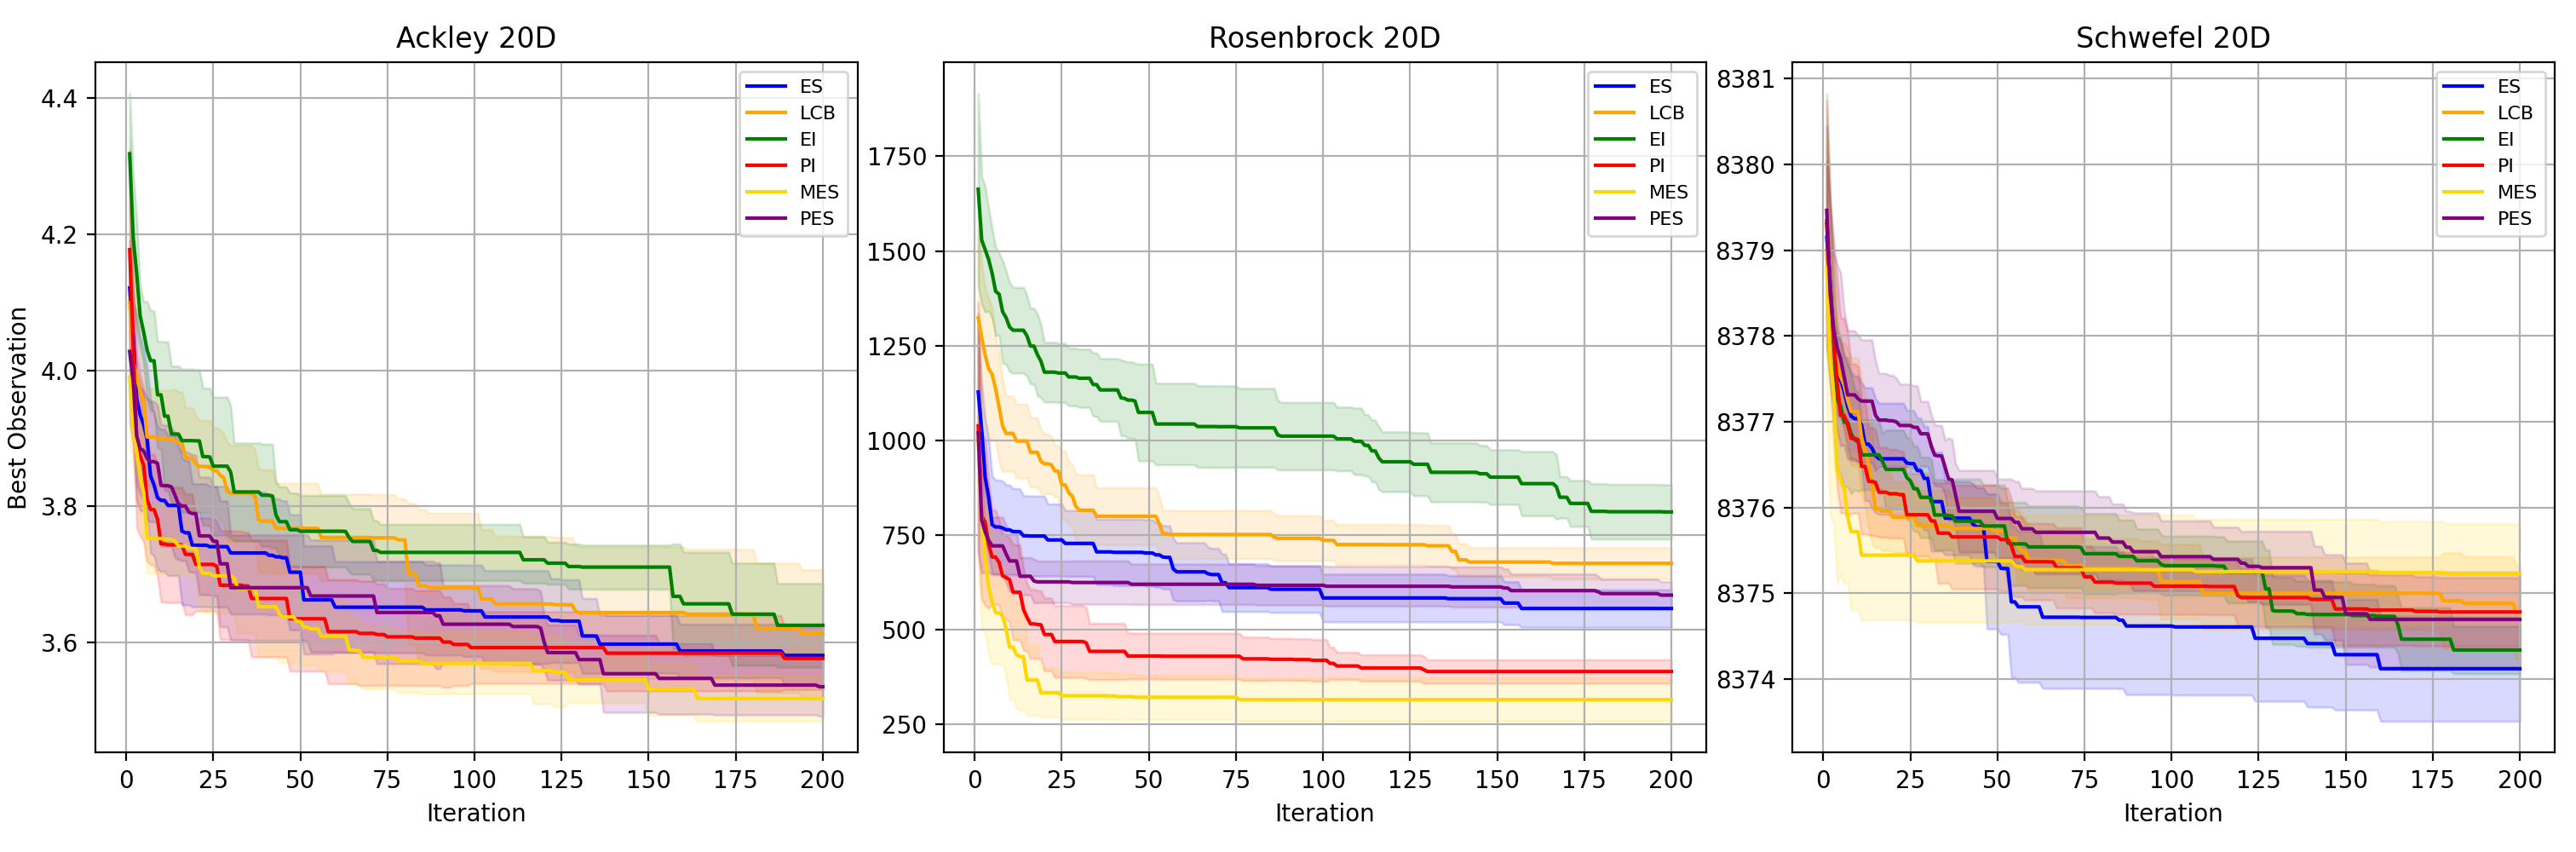
\includegraphics[width=\textwidth]{across_function.png}
    \caption[20-Dimension benchmark comparison of acquisition functions]{
        Performance comparison of six acquisition functions (ES, LCB, EI, PI, MES, PES) on three 20-dimensional benchmark functions: Ackley, Rosenbrock, and Schwefel.
        Each curve shows the median best function value found so far, with shaded areas representing 95\% confidence interval.
    }
    \label{fig:benchmark_20d}
\end{figure}

We evaluate acquisition functions on three 20-dimensional benchmark functions: Ackley, Rosenbrock, and Schwefel. Figure~\ref{fig:benchmark_20d} presents the best observed values over 200 iterations, averaged across trials, with shaded regions representing 95\% confidence interval. 

Across all cases, PES and MES exhibit consistently strong performance, characterized by a \textit{steep initial decline} and \textit{faster convergence} compared to standard baselines.

On the \textit{Ackley function}, all methods show rapid early improvement, but PES and MES achieve lower final objective values with reduced variance, indicating both efficiency and stability.

The \textit{Rosenbrock function}, known for its narrow curved valley, further highlights the advantage of entropy-based methods. PES achieves the best results, maintaining steady improvement where methods like EI and PI stagnate early.

On the more deceptive \textit{Schwefel function}, convergence is slower overall. Nonetheless, PES and MES remain competitive, achieving better final values than EI, PI, and LCB, while ES performs well but with more variability.

These results reinforce the scalability of entropy-based acquisitions. Their ability to model global uncertainty leads to \textit{faster and more reliable convergence}, especially in complex, high-dimensional landscapes.

\chapter{Concluding Remarks}

\section{Conclusion}
We conducted a systematic evaluation of six acquisition functions, LCB, EI, PI, ES, PES, and MES, within a unified BO framework, focusing on both convergence behavior and scalability. Experiments were performed across multiple benchmark functions (Ackley, Rosenbrock, Schwefel) and dimensionalities (5D, 10D, 20D), using GP surrogates trained with exact marginal log likelihood and acquisition optimization based on pre-filtered candidate sets.

Entropy-based methods, PES and MES, consistently outperformed standard baselines. They exhibited accelerated convergence, especially in the early iterations, and maintained superior performance in higher dimensions. This advantage was most prominent in the Rosenbrock and Schwefel functions, where traditional methods stagnated or displayed high variance.

The improved performance of PES and MES stems from their ability to explicitly model and reduce global uncertainty via information-theoretic criteria. Unlike myopic utility-based acquisitions such as EI or PI, entropy-based strategies promote exploration in informative regions of the search space, leading to more efficient use of evaluation budgets.

These results confirm that entropy-based acquisition functions are highly effective for high-dimensional BO, offering both scalability and robustness in navigating complex landscapes.

\section{Future Work}
An important direction for future work is the integration of hyperparameter optimization into the BO framework. While this study used fixed GP hyperparameters, optimizing them, either via marginal likelihood with advanced priors or fully Bayesian approaches, can improve surrogate accuracy and acquisition effectiveness, especially in noisy or high-dimensional regimes.

Moreover, if time permits, we aim to extend this work to the setting of optimization under uncertainty, where GP models may be employed to represent robustness metrics. 

Future work may explore the use of these acquisition strategies to guide optimization in the presence of uncertain or robustness-sensitive objectives, potentially improving the reliability and generalizability of BO in practical, high-stakes scenarios.

\bibliographystyle{IEEEtran}
\bibliography{references}
\end{document}
